\subsection{Tip i slojevi arhitekture}
Na osnovu prethodno navedene analize, odabrana je klijent-server arhitektura i aplikacija se sastoji iz 3 sloja:
\begin{enumerate}
\item Prezentacioni sloj
\item Logički sloj
\item Sloj podataka
\end{enumerate}

\subsubsection{Prezentacioni sloj}

Ovo je najviši sloj aplikacije i njegova uloga je prikazivanje korisniku vizuelnog sadržaja,
koristeći podatke koje dobija od nižeg sloja.
Zadužen je da korisniku obezbedi što lakšu i efikasniju upotrebu aplikacije.
Funkcionalnosti koje pruža razlikuju se u zavisnosti od uloge korisnika i pokrivaju najvažnije slučajeve upotrebe 
Čine ga komponente koje korisnik vidi i sa kojima interaguje kroz veb pregledač i to su:

\begin{itemize}
    \item Registracija
    \item Prijavljivanje
    \item Odabir termina za praktični i teorijski ispit
\end{itemize}


\subsubsection{Logički sloj}

Logički sloj je središnji sloj i on se sastoji od Klijentskog kontrolera i Serverskog kontrolera.
Primarni zadatak klijentskog kontrolera jeste pouzdana komunikacija sa serverskim slojem sistema. 
Još jedan njegov zadatak je prosleđivanje podataka prezentacionom sloju, kako bi on prikazao korisniku vizuelni sadržaj.
Njegove komponente su sledeće:

\begin{itemize}
    \item Autorizacija i autentifikacija
    \item Dohvatanje podataka sa servera
    \item Validacija korisničkih podataka
\end{itemize}


Zadatak serverskog kontrolera je sličan kao kod klijentskog, s tim što se ovde vrši dodatna autentifikacija 
i autorizacija. To je omogućeno jer ovoj komponenti nemaju pristup klijenti i time se postiže bezbednost.
Takođe, ovde se vrši komunikacija sa bazom podataka.
Njegove komponente su sledeće:

\begin{itemize}
    \item Autorizacija i autentifikacija
    \item Dohvatanje podataka
    \item Pregled i izmene podataka 
\end{itemize}

\subsubsection {Sloj podataka}

Baza podataka čuva sve podatke koji su neophodni za sistem i ona je kao komponenta deo ovog sloja.
Takođe, ovaj sloj sadrži i sve neophodne mehanizme za pristup bazi podataka.
Opis baze podataka se nalazi u sekciji \ref{sec:database}.


\begin{figure}[H]
  \begin{center}
      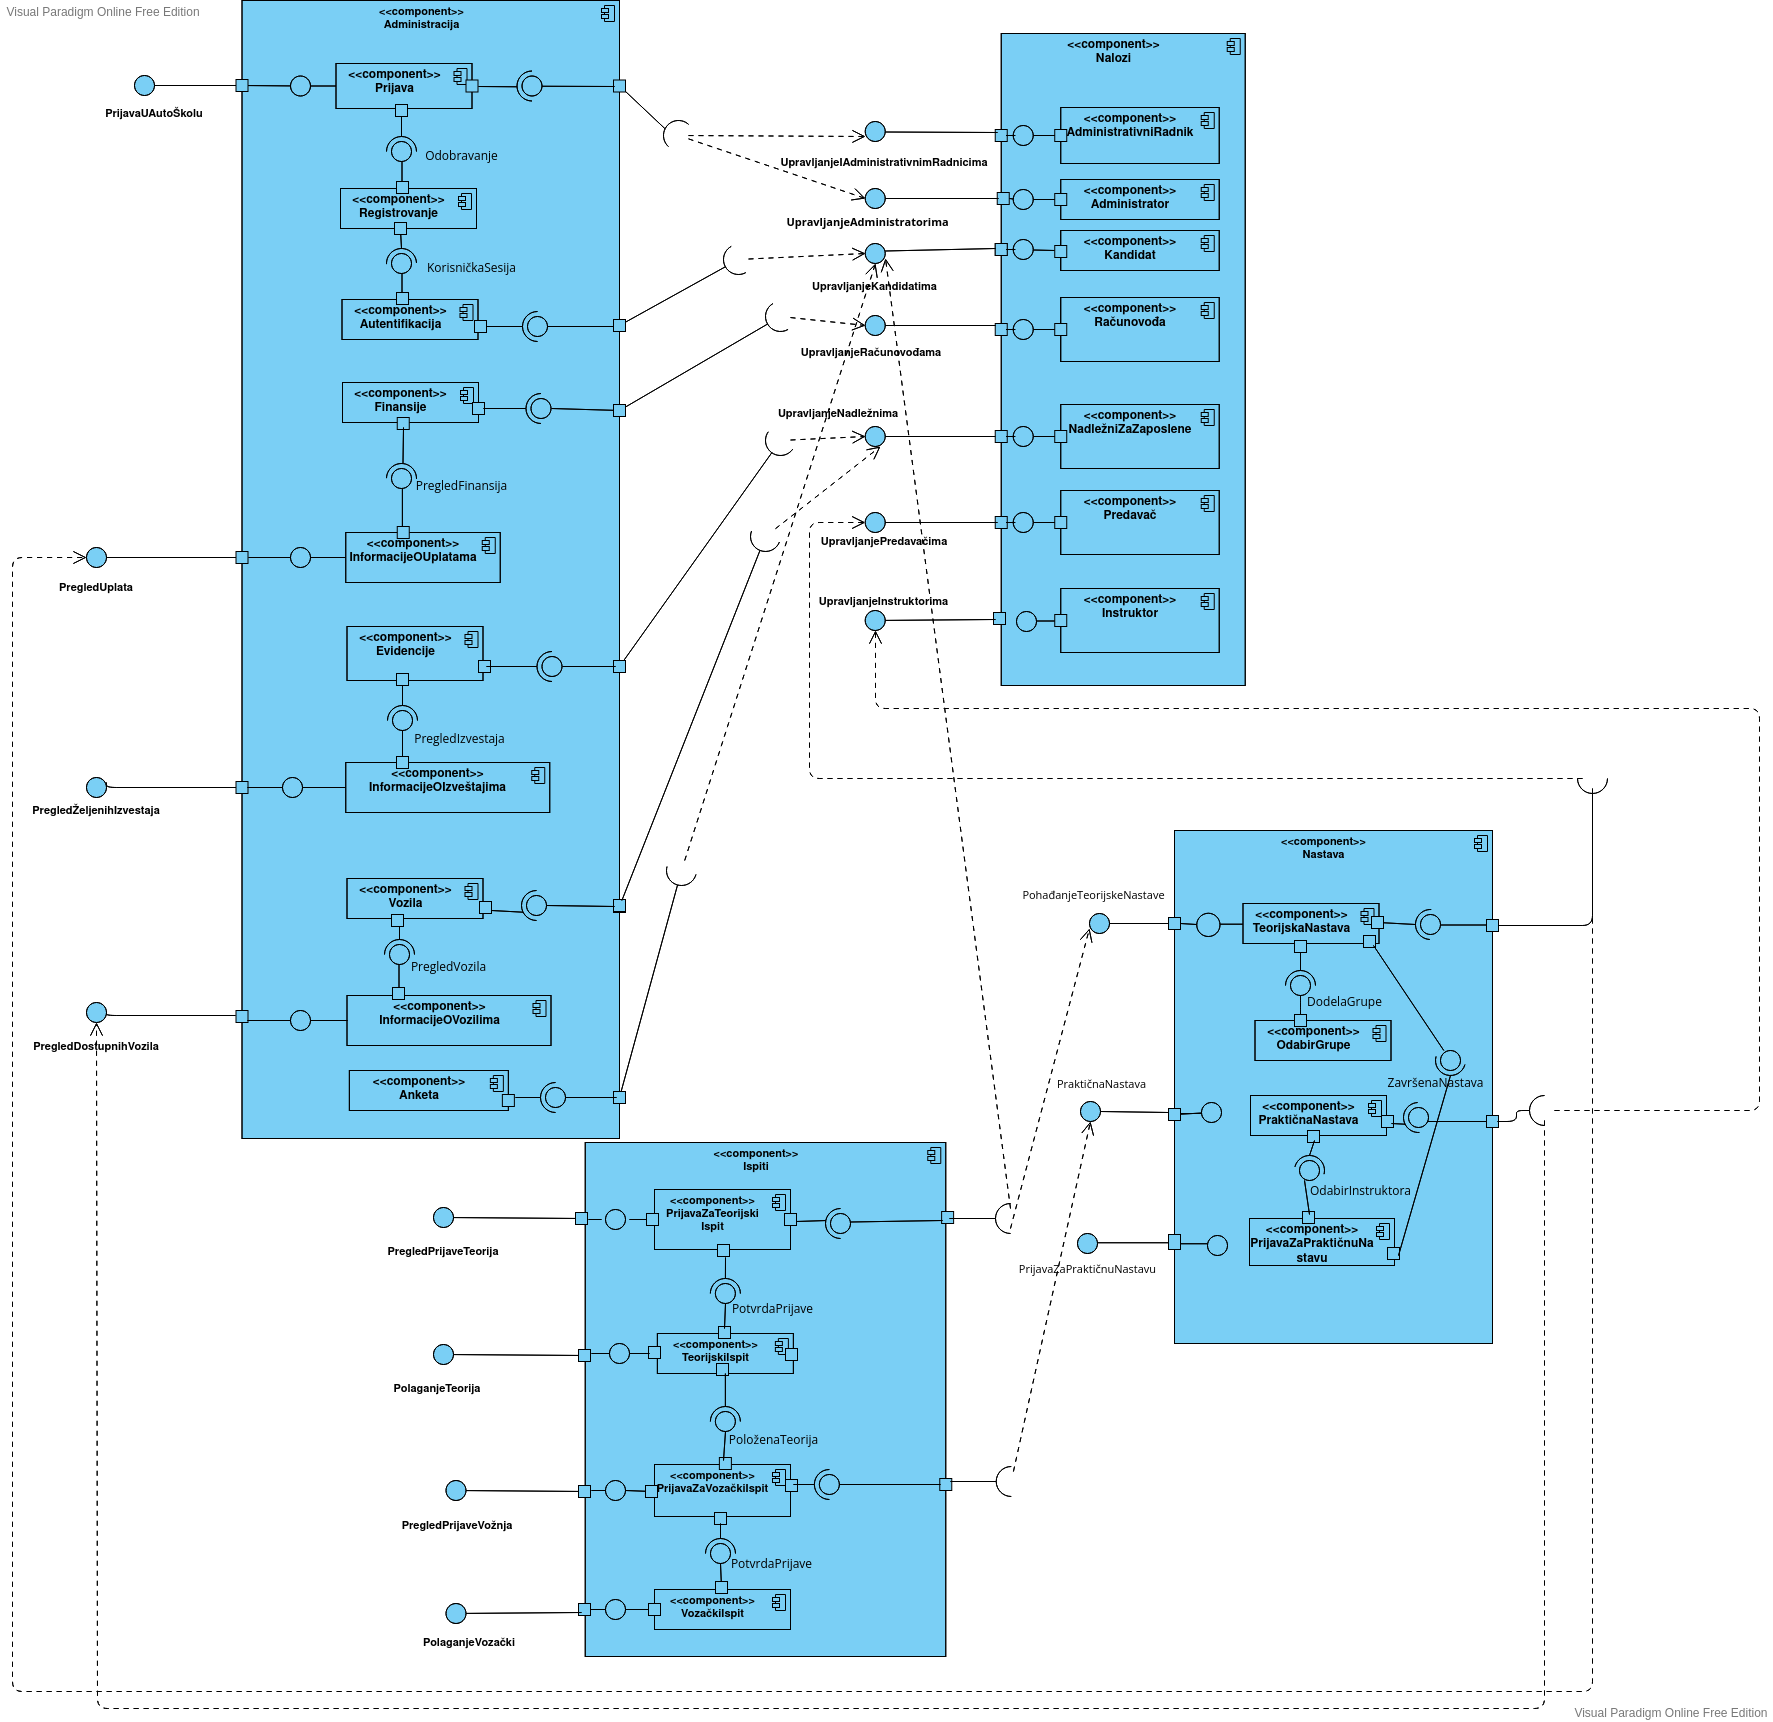
\includegraphics[width=\textwidth, height=600px]{Diagrams/dijagram_komponenti.png}
  \end{center}
  \caption {Dijagram komponenti}
  \label{dijagram_komponenti}

\end{figure}



\begin{figure}[H]
    \begin{center}
        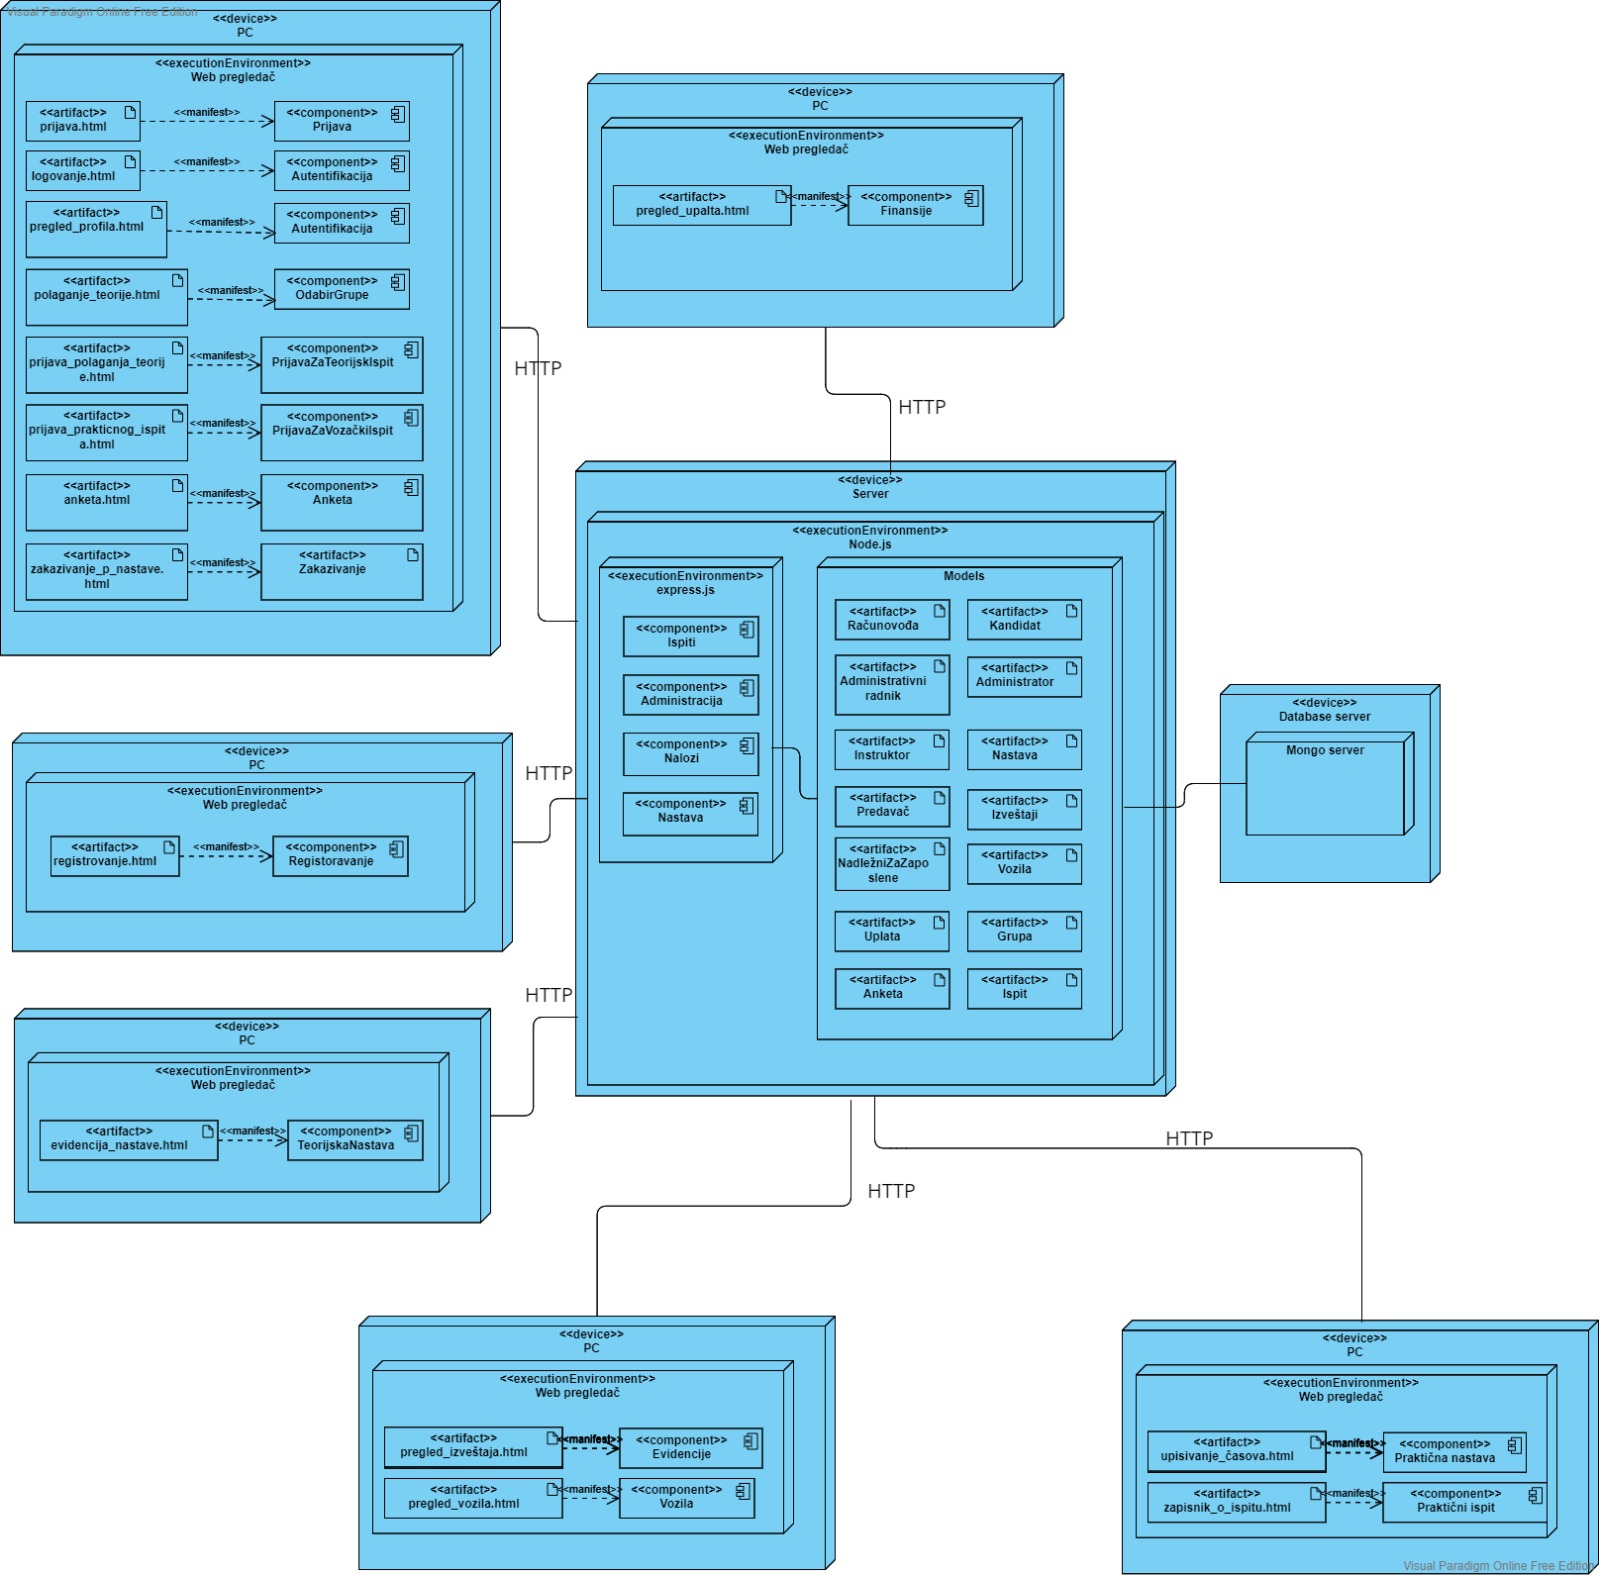
\includegraphics[width=\textwidth, height=700px]{Diagrams/dijagram_isporucivanja.jpeg}
    \end{center}
    \caption {Dijagram isporučivanja}
    \label{dijagram_isporučivanja}
  
  \end{figure}

  \newpage
